      
               
                \begin{ledgroupsized}[r]{120mm}
                \footnotesize 
                \pstart                
                \noindent\textbf{\"{U}berlieferung:}   
                \pend
                \end{ledgroupsized}
            
              
                            \begin{ledgroupsized}[r]{114mm}
                            \footnotesize 
                            \pstart \parindent -6mm
                            \makebox[6mm][l]{\textit{L}}Konzept: LH XXXVIII Bl. 144. 1 Bl. 24 x 15 cm. 1 S. An der linken und unteren Seite beschnitten. Zeichnung links oben, Text umlaufend, R\"{u}ckseite leer.\\Cc 2, Nr. 949 \pend
                            \end{ledgroupsized}
                %\normalsize
                \vspace*{5mm}
                \begin{ledgroup}
                \footnotesize 
                \pstart
            \noindent\footnotesize{\textbf{Datierungsgr\"{u}nde}: Die Datierung ergibt sich aus Leibniz' Notiz in der 2. Zeile unseres Textes. Es ist anzunehmen, dass Fouchers Mitteilung \"{u}ber den Versuch zur Bestimmung der Schwere der Luft und Leibniz' Niederschrift zeitlich nahe beieinander liegen. Das Datum April 1675 bezeichnet daher auch die Entstehungszeit des Textes.}
                \pend
                \end{ledgroup}
            
                \vspace*{8mm}
                \pstart 
                \normalsize
            \centering [144 r\textsuperscript{o}] \selectlanguage{french}Experience de Mons. l'Abb\'{e} Foucher\protect\index{Namensregister}{\textso{Foucher} (Foucherius), Simon 1644\textendash 1696}, de Dijon\protect\index{Ortsregister}{Dijon}\\ qu'il m'a dit l'an 1675. Mois d'Auril. \pend \vspace{1.0ex} \pstart  L'air estant rarifi\'{e} \`{a} un certain point diminue beaucoup de pesanteur\protect\index{Sachverzeichnis}{pesanteur!de l'air}, et est extrement leger; c'est \`{a} dire il diminue plus en pesanteur, qu'il n'augmente en volume, ou qu'il ne diminue en masse. \pend \pstart Ou la legeret\'{e} au commencement s'augmente plus que la rarefaction; et cela va jusqu'\`{a} un  certain point; mais par apres la rarefaction augmente plus que la legeret\'{e}.\selectlanguage{latin}\pend \pstart A 1. Aer inclusus. Separatus ab externo gutta aquae alteriusve liquoris. Tubus sigillatus in \textit{A} apertus  in \textit{B} horizonti parallelus, quo minus aquae pondus ad  rem pertineat, \edtext{forte rectius \textit{A} in summo \textit{B} in 1\textsuperscript{mo}, ita enim aquae gutta pondere suo frictionem pensabit neque in planitiem exporrigetur}{\lemma{}\Afootnote{forte [...] exporrigetur \textit{ erg.} \textit{ L}}} frictio quoque exigua est ob guttae  parvitatem. Jam ex toto vase \textit{CDE}, vacuo, et clauso  extrahatur  aer sugendo. Tubus \textit{AB} erit rarefactionis  index, nam cum  aer inclusus \edtext{inter \textit{A} extremum Tubi sigillatum, et \textso{guttam \textit{F}}}{\lemma{inter \textit{A}}\Afootnote{ \textit{ (1) }\ et \textit{F} guttam \textit{ (2) }\ extremum [...] \textso{\textit{F}} \textit{ L}}} ejusdem sit consistentiae cum  aere reliquo  vasis, hinc ubi spatium \textit{AF} sequens primi duplum erit aer \edtext{vasis}{\lemma{aer}\Afootnote{ \textit{ (1) }\ tubi \textit{ (2) }\ vasis \textit{ L}}} quoque duplo rarior erit, ponamus tunc 4 granis diminui pondus vasis  totius ob  aerem ex eo extractum. Ergo si duplo amplius rarefeceris, id est si gutta \textit{F} a nota 2. ad notam 4 (ponemus  enim indices notas tubo ascriptas) processerit, \edtext{utique quadrupla}{\lemma{utique}\Afootnote{ \textit{ (1) }\ duplo major \textit{ (2) }\ quadrupla \textit{ L}}} erit aeris rarefactio, seu aer \edtext{perdidit}{\lemma{aer}\Afootnote{ \textit{ (1) }\ qui restat \textit{ (2) }\ perdidit \textit{ L}}} \edtext{suae massae tres quartas}{\lemma{perdidit}\Afootnote{ \textit{ (1) }\ duas tertias \textit{ (2) }\ suae massae tres quartas \textit{ L}}}, seu quadruplum prioris spatii occupat, \edtext{quare}{\lemma{occupat,}\Afootnote{ \textit{ (1) }\ ergo \textit{ (2) }\ quare \textit{ L}}} cum diminutio ponderis extracto  aeris dimidio sit 4 \edtext{granorum, ideo}{\lemma{granorum,}\Afootnote{ \textit{ (1) }\ ergo \textit{ (2) }\ ideo \textit{ L}}} extractis tribus quartis deberet esse diminutio non 8 granorum, ut dixerat Dominus Foucherius\protect\index{Namensregister}{\textso{Foucher} (Foucherius), Simon 1644\textendash 1696} \edtext{lapsu credo memoriae}{\lemma{}\Afootnote{lapsu credo memoriae \textit{ erg.} \textit{ L}}}, sed granorum $2-4-3 \sqcap\ \displaystyle\frac{4,3}{2} \sqcap\ 6 $\rule[-4mm]{0mm}{10mm} et tamen quod est mirum diminutio fuit \edtext{granorum 10}{\lemma{granorum}\Afootnote{ \textit{ (1) }\ 8 \textit{ (2) }\ 10 \textit{ L}}}. et cum aer octuplum sui spatium occupat, utique aer extractus erit totius materiae \edtext{}{\lemma{}\Afootnote{materiae  \textbar\ pars \textit{ gestr.}\ \textbar\ $\displaystyle\frac{7}{8}$\protect\rule[-3mm]{0mm}{8mm}. \textit{ L}}} $\displaystyle\frac{7}{8}$\rule[-4mm]{0mm}{10mm}. Jam $\displaystyle\frac{4}{8}$\rule[-4mm]{0mm}{10mm} dant 4 quantum $\displaystyle\frac{7}{8}$\rule[-4mm]{0mm}{10mm} debet diminutio esse granorum 7. \edtext{(non 16 ut dixerat Dominus Foucherius) et tamen illa reperitur granorum 22}{\lemma{7.}\Afootnote{ \textit{ (1) }\ et tamen illa est granorum \textit{ (2) }\ (non 16 [...] granorum 22 \textit{ L}}}. Et ita usque ad certum punctum fit major debita diminutio. Addit ille post illud punctum non amplius ita crescere, sed rursus diminui. Difficile est rem bene experiri, ob pondus aquae. Nam si \edtext{gutta descendit}{\lemma{si}\Afootnote{ \textit{ (1) }\  gutta 8 \textit{ (2) }\ gutta descendit \textit{ L}}} rarefacto aere, pondus\protect\index{Sachverzeichnis}{pondus!aeris} ejus premet aerem exteriorem, et aer internus erit nimis rarus; sin descendit contra. Sin  horizontalis sit tubus non habebit formam guttae, sed expandet sese, nisi angustus admodum sit tubus, et gutta longissima  quo casu nocebit frictio, est ergo nonnihil difficultatis in exacto experimenti calculo.\pend 
%Zeitz auskommentiert            \newpage
%              \begin{center}                   
%              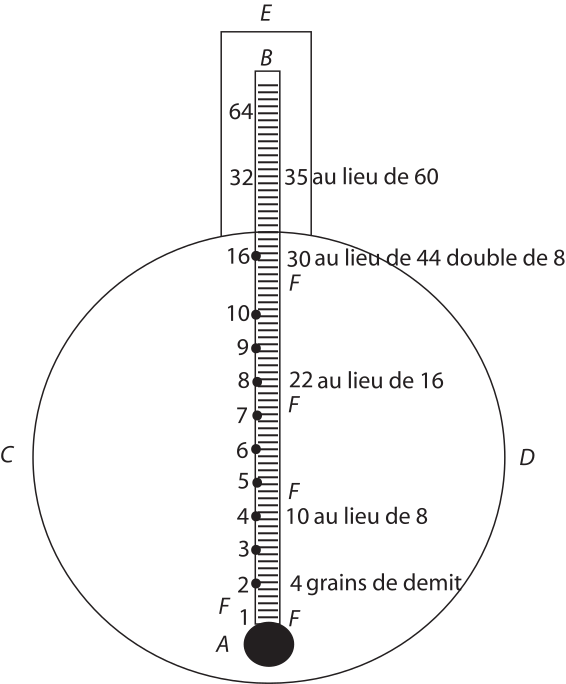
\includegraphics[width=0.65\textwidth]{images/38_144r}\\\textit{[Fig. 1]}
%              \end{center}